\documentclass[12pt,a4paper]{article}
\usepackage[utf8]{inputenc}
\usepackage[margin=1in]{geometry}
\usepackage{amsmath}
\usepackage{amsfonts}
\usepackage{amssymb}
\usepackage{graphicx}
\usepackage{listings}
\usepackage{xcolor}
\usepackage{fancyhdr}
\usepackage{titlesec}

% SQL syntax highlighting
\lstdefinestyle{sqlstyle}{
    language=SQL,
    basicstyle=\ttfamily\small,
    keywordstyle=\color{blue}\bfseries,
    commentstyle=\color{green!50!black},
    stringstyle=\color{red},
    numbers=left,
    numberstyle=\tiny\color{gray},
    numbersep=5pt,
    breaklines=true,
    breakatwhitespace=true,
    tabsize=2,
    showspaces=false,
    showstringspaces=false,
    frame=single,
    rulecolor=\color{gray!30},
    backgroundcolor=\color{gray!5}
}

\lstset{style=sqlstyle}

% Page setup
\pagestyle{fancy}
\fancyhf{}
\rhead{CSE 414 - Assignment 04}
\lhead{Oracle SQL Practice}
\cfoot{\thepage}

% Title formatting
\titleformat{\section}{\Large\bfseries}{}{0em}{}
\titleformat{\subsection}{\large\bfseries}{}{0em}{}

\begin{document}

% Title Page
\begin{titlepage}
    \begin{figure}[htbp]
    \centering
    
\includegraphics[width=0.2\textwidth]{cu.png}
    \end{figure}
    \centering
    \vspace*{0.5cm}
    {\Huge\bfseries University of Chittagong}\\[0.5cm]
    {\Large Department of Computer Science \& Engineering}\\[0.5cm]
    {\large Database Systems Lab}\\[2cm]
    
    {\large Name of the assignment:}\\[0.3cm]
    {\LARGE\bfseries Chapters 8, 9, 10 \& 18 Practice Problems}\\[0.5cm]
    {\large CSE 414}\\[0.5cm]
    {\large Assignment 04}\\[3cm]
    
    \begin{minipage}[t]{0.4\textwidth}
    \raggedleft
    Submitted By:\\
    \large \textbf{Debashish Chakraborty}\\
    \large ID: 23701034
    \end{minipage}
    \hspace{0.05\textwidth}
    \vrule width 1pt
    \hspace{0.05\textwidth}
    \begin{minipage}[t]{0.4\textwidth}
    Submitted To:\\
    \large \textbf{Dr. Rudra Pratap Deb Nath}\\
    \large Associate Professor
    \end{minipage}
    
    \vfill
    {\large June 14, 2025}
\end{titlepage}

\newpage
\tableofcontents
\newpage 

\section{Practice 8 (Solutions)}
\begin{itemize}
    \item \textit{INSERT data into the MY\_EMPLOYEE table.}

\subsection*{8.1}
\textbf{Problem:} Run the statement in the lab8\_1.sql script to build the MY\_EMPLOYEE table that will be used for the lab.

\textbf{Solution:}
\begin{lstlisting}
CREATE TABLE my_employee ( 
    ID NUMBER(4)
    CONSTRAINT MY_EMPLOYEE_ID_NN NOT NULL,
    LAST_NAME VARCHAR2(25),
    FIRST_NAME VARCHAR2(25),
    USERID VARCHAR2(8),
    SALARY NUMBER(9, 2)
);
\end{lstlisting}

\subsection*{8.2}
\textbf{Problem:} Describe the structure of the MY\_EMPLOYEE table to identify the column names.
\\
\begin{figure}[htbp]
  \centering
  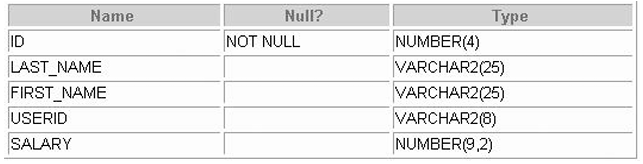
\includegraphics[width=0.8\textwidth]{Screenshots/82.png}
\end{figure}\\
\textbf{Solution:}
\begin{lstlisting}
DESCRIBE my_employee;
\end{lstlisting}

\subsection*{8.3}
\textbf{Problem:} Add the first row of data to the MY\_EMPLOYEE table from the following sample data. Do not list the columns in the INSERT clause.
\\
\begin{figure}[htbp]
  \centering
  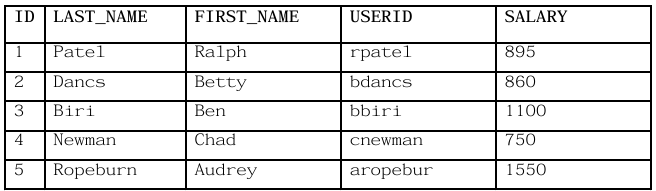
\includegraphics[width=0.8\textwidth]{Screenshots/83.png}
\end{figure}\\
\textbf{Solution:}
\begin{lstlisting}
INSERT INTO MY_EMPLOYEE VALUES ( 1, 
    'Patel',
    'Ralph',
    'rpatel',
    895 );
\end{lstlisting}

\subsection*{8.4}
\textbf{Problem:} Populate the MY\_EMPLOYEE table with the second row of sample data from the preceding list. This time, list the columns explicitly in the INSERT clause.

\textbf{Solution:}
\begin{lstlisting}
INSERT INTO MY_EMPLOYEE ( 
    ID,
    LAST_NAME,
    FIRST_NAME,
    USERID,
    SALARY
) VALUES ( 2,
    'Dancs',
    'Betty',
    'bdancs',
    860 );
\end{lstlisting}

\subsection*{8.5}
\textbf{Problem:} Confirm your addition to the table.
\\
\begin{figure}[htbp]
  \centering
  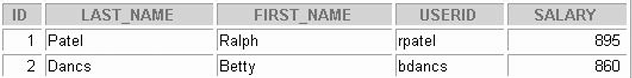
\includegraphics[width=0.8\textwidth]{Screenshots/85.png}
\end{figure}\\
\textbf{Solution:}
\begin{lstlisting}
SELECT 
    *
FROM
    my_employee;
\end{lstlisting}
\newpage
\subsection*{8.6}
\textbf{Problem:} Write an insert statement in a text file named loademp.sql to load rows into the MY\_EMPLOYEE table. Concatenate the first letter of the first name and the first seven characters of the last name to produce the userid.

\textbf{Solution:}
\begin{lstlisting}

INSERT INTO my_employee VALUES ( &p_id,
    '&p_last_name',
    '&p_first_name',
    lower(substr('&p_first_name', 1, 1)
    || substr('&p_last_name', 1, 7)),
    &p_salary );

\end{lstlisting}

\subsection*{8.7}
\textbf{Problem:} Populate the table with the next two rows of sample data by running the INSERT statement in the script that you created.

\textbf{Solution:}
\begin{lstlisting}

INSERT INTO my_employee VALUES ( &p_id,
    '&p_last_name',
    '&p_first_name',
    lower(substr('&p_first_name', 1, 1)
    || substr('&p_last_name', 1, 7)),
    &p_salary );


\end{lstlisting}

\subsection*{8.8}
\textbf{Problem:} Confirm your additions to the table.
\\
\begin{figure}[htbp]
  \centering
  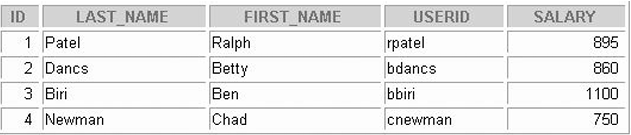
\includegraphics[width=0.8\textwidth]{Screenshots/88.png}
\end{figure}\\
\textbf{Solution:}
\begin{lstlisting}
SELECT 
    *
FROM
    my_employee;
\end{lstlisting}

\subsection*{8.9}
\textbf{Problem:} Make the data additions permanent. Update and delete data in the MY\_EMPLOYEE table.

\textbf{Solution:}
\begin{lstlisting}
COMMIT;
\end{lstlisting}
\item \textit{UPDATE and DELETE data in the MY\_EMPLOYEE table.}
\subsection*{8.10}
\textbf{Problem:} Change the last name of employee 3 to Drexler.

\textbf{Solution:}
\begin{lstlisting}
UPDATE my_employee 
SET
    last_name = 'Drexler'
WHERE
    id = 3;
\end{lstlisting}

\subsection*{8.11}
\textbf{Problem:} Change the salary to 1000 for all employees with a salary less than 900.

\textbf{Solution:}
\begin{lstlisting}
UPDATE my_employee 
SET
    salary = 1000
WHERE
    salary < 900;
\end{lstlisting}

\subsection*{8.12}
\textbf{Problem:} Verify your changes to the table.
\\
\begin{figure}[htbp]
  \centering
  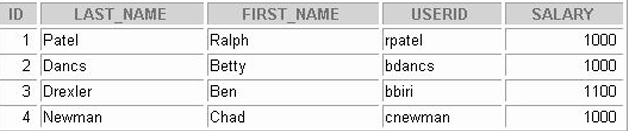
\includegraphics[width=0.8\textwidth]{Screenshots/812.png}
\end{figure}\newpage
\textbf{Solution:}
\begin{lstlisting}
SELECT 
    last_name,
    salary
FROM
    my_employee;
\end{lstlisting}

\subsection*{8.13}
\textbf{Problem:} Delete Betty Dancs from the MY\_EMPLOYEE table.

\textbf{Solution:}
\begin{lstlisting}
DELETE FROM my_employee 
WHERE
    last_name = 'Dancs';
\end{lstlisting}

\subsection*{8.14}
\textbf{Problem:} Confirm your changes to the table.
\\
\begin{figure}[htbp]
  \centering
  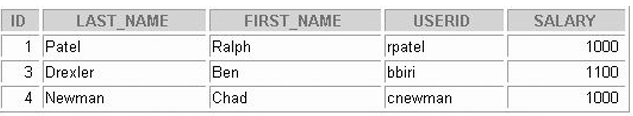
\includegraphics[width=0.8\textwidth]{Screenshots/814.png}
\end{figure}\\
\textbf{Solution:}
\begin{lstlisting}
SELECT 
    *
FROM
    my_employee;
\end{lstlisting}

\subsection*{8.15}
\textbf{Problem:} Commit all pending changes. Control data transaction to the MY\_EMPLOYEE table.

\textbf{Solution:}
\begin{lstlisting}
COMMIT;
\end{lstlisting}\\
\newpage
\item \textit{Control data transaction to the MY\_EMPLOYEE table.}
\subsection*{8.16}
\textbf{Problem:} Populate the table with the last row of sample data by modifying the statements in the script that you created in step 6. Run the statements in the script.

\textbf{Solution:}
\begin{lstlisting}

INSERT INTO my_employee VALUES ( &p_id,
    '&p_last_name',
    '&p_first_name',
    lower(substr('&p_first_name', 1, 1)
    || substr('&p_last_name', 1, 7)),
    &p_salary );

\end{lstlisting}

\subsection*{8.17}
\textbf{Problem:} Confirm your addition to the table.
\\
\begin{figure}[htbp]
  \centering
  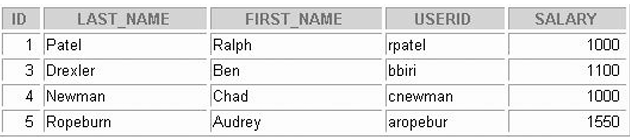
\includegraphics[width=0.6\textwidth]{Screenshots/817.png}
\end{figure}\\
\textbf{Solution:}
\begin{lstlisting}
SELECT 
    *
FROM
    my_employee;
\end{lstlisting}

\subsection*{8.18}
\textbf{Problem:} Mark an intermediate point in the processing of the transaction.

\textbf{Solution:}
\begin{lstlisting}
SAVEPOINT step_18;
\end{lstlisting}

\subsection*{8.19}
\textbf{Problem:} Empty the entire table.

\textbf{Solution:}
\begin{lstlisting}
DELETE FROM my_employee;
\end{lstlisting}

\subsection*{8.20}
\textbf{Problem:} Confirm that the table is empty.

\textbf{Solution:}
\begin{lstlisting}
SELECT 
    *
FROM
    my_employee;
\end{lstlisting}

\subsection*{8.21}
\textbf{Problem:} Discard the most recent DELETE operation without discarding the earlier INSERT operation.

\textbf{Solution:}
\begin{lstlisting}
ROLLBACK TO step_18;
\end{lstlisting}

\subsection*{8.22}
\textbf{Problem:} Confirm that the new row is still intact.
\\
\begin{figure}[htbp]
  \centering
  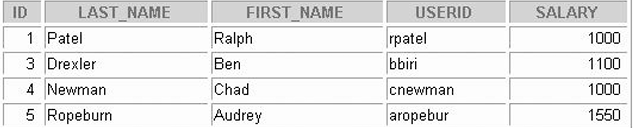
\includegraphics[width=0.8\textwidth]{Screenshots/822.png}
\end{figure}\\
\textbf{Solution:}
\begin{lstlisting}
SELECT 
    *
FROM
    my_employee;
\end{lstlisting}

\subsection*{8.23}
\textbf{Problem:} Make the data addition permanent.

\textbf{Solution:}
\begin{lstlisting}
COMMIT;
\end{lstlisting}
\newpage
\section{Practice 9 (Solutions)}
\item \textit{Create, Alter, Drop, Rename, Truncate and adding Comment to a table.} 
\subsection*{9.1}
\textbf{Problem:} Create the DEPT table based on the following table instance chart. Place the syntax in a script called lab9\_1.sql, then execute the statement in the script to create the table. Confirm that the table is created.
\\
\begin{figure}[htbp]
  \centering
  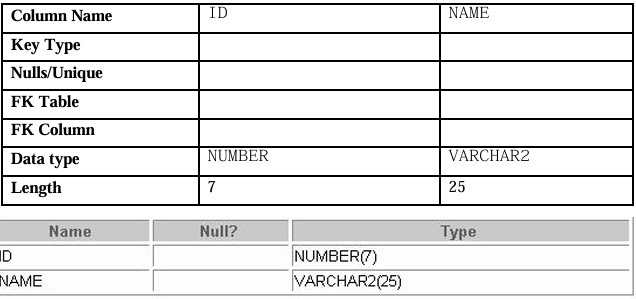
\includegraphics[width=0.8\textwidth]{Screenshots/91.png}
\end{figure}\\
\textbf{Solution:}
\begin{lstlisting}
CREATE TABLE dept ( 
    id NUMBER(7),
    name VARCHAR2(25)
);
-- Verification
DESCRIBE dept;
\end{lstlisting}

\subsection*{9.2}
\textbf{Problem:} Populate the DEPT table with data from the DEPARTMENTS table. Include only columns that you need.

\textbf{Solution:}
\begin{lstlisting}
INSERT INTO dept 
SELECT
    department_id,
    department_name
FROM
    departments;
\end{lstlisting}

\subsection*{9.3}
\textbf{Problem:} Create the EMP table based on the following table instance chart. Place the syntax in a script called lab9\_3.sql, and then execute the statement in the script to create the table. Confirm that the table is created.
\\
\begin{figure}[htbp]
  \centering
  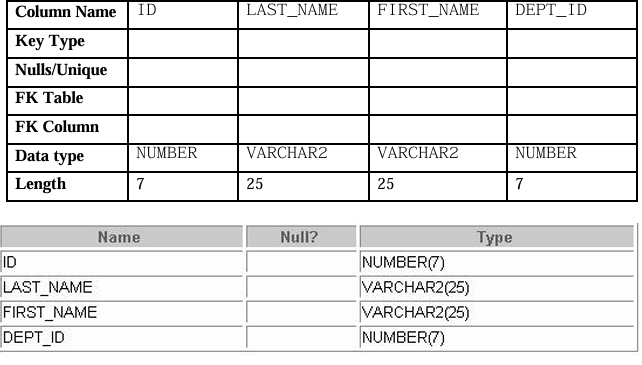
\includegraphics[width=0.8\textwidth]{Screenshots/93.png}
\end{figure}\\
\textbf{Solution:}
\begin{lstlisting}
CREATE TABLE emp (
    id number(7),
    last_name varchar2(25),
    first_name varchar2(25),
    dept_id number(7)
);

-- Verification
DESCRIBE emp;
\end{lstlisting}

\subsection*{9.4}
\textbf{Problem:} Modify the EMP table to allow for longer employee last names. Confirm your modification.
\\
\begin{figure}[htbp]
  \centering
  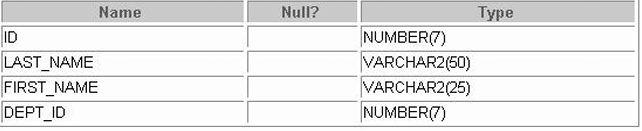
\includegraphics[width=0.8\textwidth]{Screenshots/94.png}
\end{figure}\\
\newpage
\textbf{Solution:}
\begin{lstlisting}
ALTER TABLE emp MODIFY ( 
    last_name VARCHAR2(50)
);
-- Verification
DESCRIBE emp;
\end{lstlisting}

\subsection*{9.5}
\textbf{Problem:} Confirm that both the DEPT and EMP tables are stored in the data dictionary. (Hint: USER\_TABLES)
\\
\begin{figure}[htbp]
  \centering
  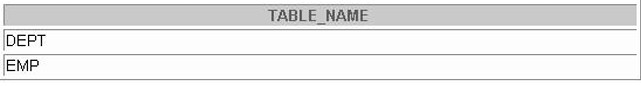
\includegraphics[width=0.8\textwidth]{Screenshots/95.png}
\end{figure}\\
\textbf{Solution:}
\begin{lstlisting}
SELECT 
    table_name
FROM
    user_tables
WHERE
    table_name IN ( 'DEPT', 'EMP' );
\end{lstlisting}

\subsection*{9.6}
\textbf{Problem:} Create the EMPLOYEES2 table based on the structure of the EMPLOYEES table. Include only the EMPLOYEE\_ID, FIRST\_NAME, LAST\_NAME, SALARY, and DEPARTMENT\_ID columns. Name the columns in your new table ID, FIRST\_NAME, LAST\_NAME, SALARY, and DEPT\_ID, respectively.

\textbf{Solution:}
\begin{lstlisting}
CREATE TABLE employees2 
AS
SELECT
    employee_id id,
    first_name,
    last_name,
    salary,
    department_id dept_id
FROM
    employees;
\end{lstlisting}

\subsection*{9.7}
\textbf{Problem:} Drop the EMP table.

\textbf{Solution:}
\begin{lstlisting}
DROP TABLE emp;
\end{lstlisting}

\subsection*{9.8}
\textbf{Problem:} Rename the EMPLOYEES2 table to EMP.

\textbf{Solution:}
\begin{lstlisting}
RENAME employees2 TO emp;
\end{lstlisting}

\subsection*{9.9}
\textbf{Problem:} Add a comment to the DEPT and EMP table definitions describing the tables. Confirm your additions in the data dictionary.

\textbf{Solution:}
\begin{lstlisting}
COMMENT ON TABLE emp IS 
    'Employee Information';

COMMENT ON TABLE dept IS
    'Department Information';

SELECT
    *
FROM
    user_tab_comments
WHERE
    table_name = 'DEPT'
    OR table_name = 'EMP';
\end{lstlisting}

\subsection*{9.10}
\textbf{Problem:} Drop the FIRST\_NAME column from the EMP table. Confirm your modification by checking the description of the table.

\textbf{Solution:}
\begin{lstlisting}
ALTER TABLE emp DROP COLUMN first_name;
-- Verification
DESCRIBE emp;
\end{lstlisting}

\subsection*{9.11}
\textbf{Problem:} In the EMP table, mark the DEPT\_ID column in the EMP table as UNUSED. Confirm your modification by checking the description of the table.

\textbf{Solution:}
\begin{lstlisting}
ALTER TABLE emp SET UNUSED ( dept_id );
-- Verification
DESCRIBE emp;
\end{lstlisting}

\subsection*{9.12}
\textbf{Problem:} Drop all the UNUSED columns from the EMP table. Confirm your modification by checking the description of the table.

\textbf{Solution:}
\begin{lstlisting}
ALTER TABLE emp DROP UNUSED COLUMNS;
-- Verification
DESCRIBE emp;
\end{lstlisting}
\newpage 
\section{Practice 10 (Solutions)}
\item \textit{Creating Constraints like NOT NULL, UNIQUE, PRIMARY KEY, FOREIGN KEY, CHECK etc.}
\subsection*{10.1}
\textbf{Problem:} Add a table-level PRIMARY KEY constraint to the EMP table on the ID column. The constraint should be named at creation. Name the constraint my\_emp\_id\_pk.

\textit{Hint: The constraint is enabled as soon as the ALTER TABLE command executes successfully.}

\textbf{Solution:}
\begin{lstlisting}
ALTER TABLE emp ADD CONSTRAINT my_emp_id_pk PRIMARY KEY (id);
\end{lstlisting}

\subsection*{10.2}
\textbf{Problem:} Create a PRIMARY KEY constraint to the DEPT table using the ID column. The constraint should be named at creation. Name the constraint my\_deptid\_pk.

\textit{Hint: The constraint is enabled as soon as the ALTER TABLE command executes successfully.}

\textbf{Solution:}
\begin{lstlisting}
ALTER TABLE dept ADD CONSTRAINT my_deptid_pk PRIMARY KEY (id);
\end{lstlisting}

\subsection*{10.3}
\textbf{Problem:} Add a column DEPT\_ID to the EMP table. Add a foreign key reference on the EMP table that ensures that the employee is not assigned to a nonexistent department. Name the constraint my\_emp\_dept\_id\_fk.

\textbf{Solution:}
\begin{lstlisting}
ALTER TABLE emp ADD ( 
    dept_id NUMBER(7)
);

ALTER TABLE emp
ADD CONSTRAINT my_emp_dept_id_fk FOREIGN KEY ( dept_id )
REFERENCES dept ( id );
\end{lstlisting}

\subsection*{10.4}
\textbf{Problem:} Confirm that the constraints were added by querying the USER\_CONSTRAINTS view. Note the types and names of the constraints. Save your statement text in a file called lab10\_4.sql.
\\
\begin{figure}[htbp]
  \centering
  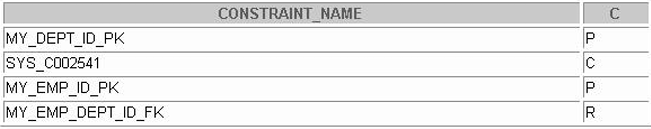
\includegraphics[width=0.8\textwidth]{Screenshots/104.png}
\end{figure}\\
\textbf{Solution:}
\begin{lstlisting}
SELECT 
    constraint_name,
    constraint_type
FROM
    user_constraints
WHERE
    table_name IN ( 'EMP', 'DEPT' );
\end{lstlisting}

\subsection*{10.5}
\textbf{Problem:} Display the object names and types from the USER\_OBJECTS data dictionary view for the EMP and DEPT tables. Notice that the new tables and a new index were created.

\textbf{Solution:}
\begin{lstlisting}
SELECT 
    object_name,
    object_type
FROM
    user_objects
WHERE
    object_name LIKE 'EMP%'
    OR object_name LIKE 'DEPT%';
\end{lstlisting}

\subsection*{10.6}
\textbf{Problem:} Modify the EMP table. Add a COMMISSION column of NUMBER data type, precision 2, scale 2. Add a constraint to the commission column that ensures that a commission value is greater than zero.

\textbf{Solution:}
\begin{lstlisting}
ALTER TABLE emp ADD commission NUMBER(2, 2) 
CONSTRAINT my_emp_comm_ck CHECK ( commission >= 0 );
\end{lstlisting}

\section{Practice 18 (Solutions)}

\subsection*{18.1}
\textbf{Problem:} Write a query to display the last name, department number, and salary of any employee whose department number and salary both match the department number and salary of any employee who earns a commission.
\\
\begin{figure}[htbp]
  \centering
  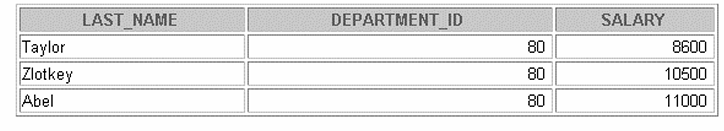
\includegraphics[width=0.8\textwidth]{Screenshots/181.png}
\end{figure}\\
\textbf{Solution:}
\begin{lstlisting}
SELECT 
    last_name,
    department_id,
    salary
FROM
    employees
WHERE
    ( salary, department_id ) IN (
        SELECT
            salary, department_id
        FROM
            employees
        WHERE
            commission_pct IS NOT NULL
    );
\end{lstlisting}

\subsection*{18.2}
\textbf{Problem:} Display the last name, department name, and salary of any employee whose salary and commission match the salary and commission of any employee located in location ID 1700.
\\
\begin{figure}[htbp]
  \centering
  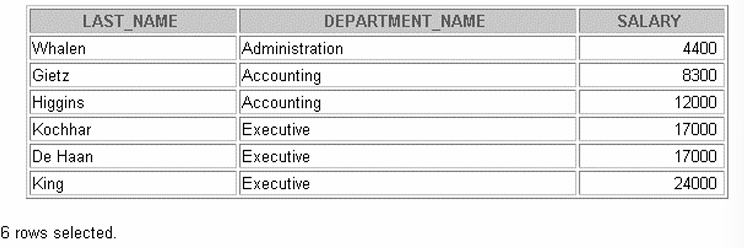
\includegraphics[width=0.8\textwidth]{Screenshots/182.png}
\end{figure}\\
\textbf{Solution:}
\begin{lstlisting}
SELECT 
    last_name,
    department_name,
    salary
FROM
    employees e,
    departments d
WHERE
    e.department_id = d.department_id
    AND ( salary, nvl(commission_pct, 0) ) IN (
        SELECT
            salary, nvl(commission_pct, 0)
        FROM
            employees e, departments d
        WHERE
            e.department_id = d.department_id
            AND d.location_id = 1700
    );
\end{lstlisting}

\subsection*{18.3}
\textbf{Problem:} Create a query to display the last name, hire date, and salary for all employees who have the same salary and commission as Kochhar.

\textit{Note: Do not display Kochhar in the result set.}
\\
\begin{figure}[htbp]
  \centering
  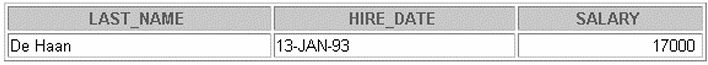
\includegraphics[width=0.8\textwidth]{Screenshots/183.png}
\end{figure}\\
\textbf{Solution:}
\begin{lstlisting}
SELECT 
    last_name,
    hire_date,
    salary
FROM
    employees
WHERE
    ( salary, nvl(commission_pct, 0) ) IN (
        SELECT
            salary, nvl(commission_pct, 0)
        FROM
            employees
        WHERE
            last_name = 'Kochhar'
    )
    AND last_name != 'Kochhar';
\end{lstlisting}

\subsection*{18.4}
\textbf{Problem:} Create a query to display the employees who earn a salary that is higher than the salary of all of the sales managers (JOB\_ID = 'SA\_MAN'). Sort the results on salary from highest to lowest.
\\
\begin{figure}[htbp]
  \centering
  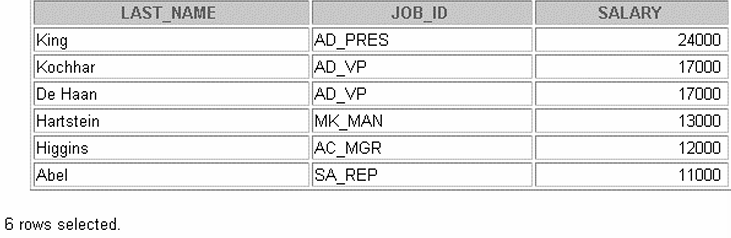
\includegraphics[width=0.8\textwidth]{Screenshots/184.png}
\end{figure}\\
\textbf{Solution:}
\begin{lstlisting}
SELECT 
    last_name,
    job_id,
    salary
FROM
    employees
WHERE
    salary > ALL (
        SELECT
            salary
        FROM
            employees
        WHERE
            job_id = 'SA_MAN'
    )
ORDER BY
    salary DESC;
\end{lstlisting}

\subsection*{18.5}
\textbf{Problem:} Display the details of the employee ID, last name, and department ID of those employees who live in cities whose name begins with T.
\\
\begin{figure}[htbp]
  \centering
  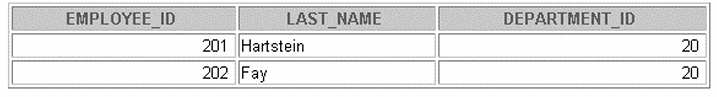
\includegraphics[width=0.8\textwidth]{Screenshots/185.png}
\end{figure}\\
\newpage
\textbf{Solution:}
\begin{lstlisting}
SELECT 
    employee_id,
    last_name,
    department_id
FROM
    employees
WHERE
    department_id IN (
        SELECT
            department_id
        FROM
            departments
        WHERE
            location_id IN (
                SELECT
                    location_id
                FROM
                    locations
                WHERE
                    city LIKE 'T%'
            )
    );
\end{lstlisting}

\subsection*{18.6}
\textbf{Problem:} Write a query to find all employees who earn more than the average salary in their departments. Display last name, salary, department ID, and the average salary for the department. Sort by average salary. Use aliases for the columns retrieved by the query as shown in the sample output.
\\
\begin{figure}[htbp]
  \centering
  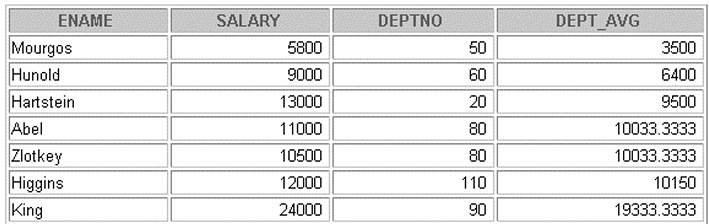
\includegraphics[width=0.8\textwidth]{Screenshots/186.png}
\end{figure}\\
\textbf{Solution:}
\begin{lstlisting}
SELECT 
    e.last_name ename,
    e.salary salary,
    e.department_id deptno,
    (SELECT AVG(salary) FROM employees WHERE department_id = e.department_id) dept_avg
FROM employees e
WHERE e.salary > (
    SELECT AVG(salary)
    FROM employees
    WHERE department_id = e.department_id
)
ORDER BY dept_avg;
\end{lstlisting}

\subsection*{18.7}
\textbf{Problem:} Find all employees who are not supervisors.
\\
\begin{figure}[htbp]
  \centering
  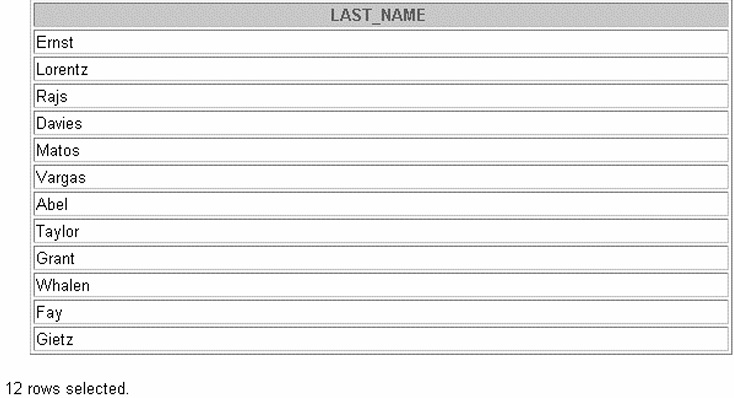
\includegraphics[width=0.8\textwidth]{Screenshots/187.png}
\end{figure}\\
\textbf{Solution:}

\textbf{a. First do this using the NOT EXISTS operator:}
\begin{lstlisting}
SELECT 
    outer.last_name
FROM
    employees outer
WHERE
    NOT EXISTS (
        SELECT
            'X'
        FROM
            employees inner
        WHERE
            inner.manager_id = outer.employee_id
    );
\end{lstlisting}
\newpage
\textbf{b. Can this be done by using the NOT IN operator:}
\begin{lstlisting}
SELECT 
    outer.last_name
FROM
    employees outer
WHERE
    outer.employee_id NOT IN (
        SELECT
            inner.manager_id
        FROM
            employees inner
    );
\end{lstlisting}

In this alternative solution, the subquery picks up a NULL value. So the entire query returns no rows. Because  all conditions that compare a NULL value result in NULL. Whenever NULL values are likely to be part of the value set, we should not use NOT IN as a substitute for NOT EXISTS.

\subsection*{18.8}
\textbf{Problem:} Write a query to display the last names of the employees who earn less than the average salary in their departments.
\\
\begin{figure}[htbp]
  \centering
  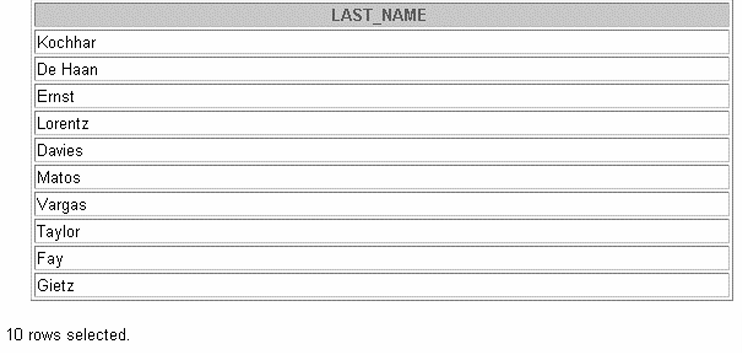
\includegraphics[width=0.6\textwidth]{Screenshots/188.png}
\end{figure}\\
\textbf{Solution:}
\begin{lstlisting}
SELECT 
    last_name
FROM
    employees outer
WHERE
    outer.salary < (
        SELECT
            AVG(inner.salary)
        FROM
            employees inner
        WHERE
            inner.department_id = outer.department_id
    );
\end{lstlisting}

\subsection*{18.9}
\textbf{Problem:} Write a query to display the last names who have one or more coworkers in their departments with later hire dates but higher salaries.
\\
\begin{figure}[htbp]
  \centering
  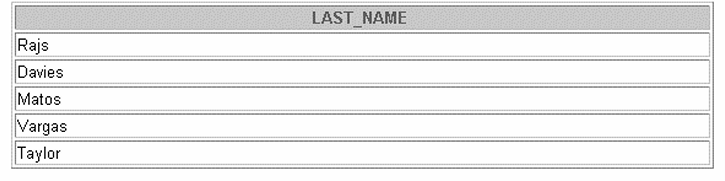
\includegraphics[width=0.8\textwidth]{Screenshots/189.png}
\end{figure}\\
\textbf{Solution:}
\begin{lstlisting}
SELECT 
    last_name
FROM
    employees outer
WHERE
    EXISTS (
        SELECT
            'X'
        FROM
            employees inner
        WHERE
            inner.department_id = outer.department_id
            AND inner.hire_date > outer.hire_date
            AND inner.salary > outer.salary
    );
\end{lstlisting}

\subsection*{18.10}
\textbf{Problem:} Write a query to display the employee ID, last names of the employees, and department names of all employees.
\textit{Note: Use a scalar subquery to retrieve the department name in the SELECT statement.}
\\
\begin{figure}[htbp]
  \centering
  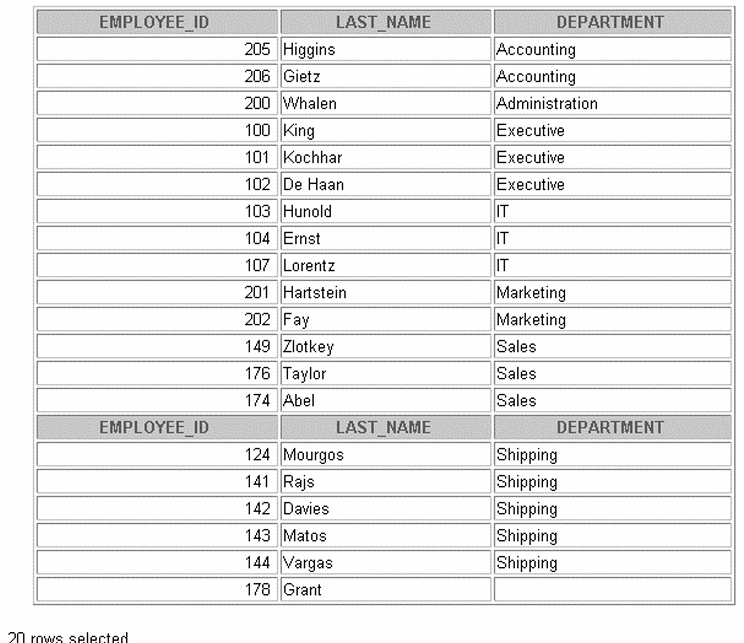
\includegraphics[width=0.5\textwidth]{Screenshots/1810.png}
\end{figure}\\
\newpage
\textbf{Solution:}
\begin{lstlisting}
SELECT 
    employee_id,
    last_name,
    (
        SELECT
            department_name
        FROM
            departments d
        WHERE
            e.department_id = d.department_id
    ) department
FROM
    employees e
ORDER BY
    department;
\end{lstlisting}

\subsection*{18.11}
\textbf{Problem:} Write a query to display the department names of those departments whose total salary cost is above one-eighth (1/8) of the total salary cost of the whole company. Use the WITH clause to write this query. Name the query SUMMARY.
\\
\begin{figure}[htbp]
  \centering
  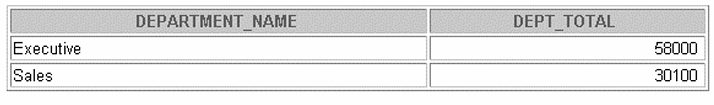
\includegraphics[width=0.8\textwidth]{Screenshots/1811.png}
\end{figure}\\
\newpage
\textbf{Solution:}
\begin{lstlisting}
WITH summary AS ( 
    SELECT
        department_name,
        SUM(salary) AS dept_total
    FROM
        employees,
        departments
    WHERE
        employees.department_id = departments.department_id
    GROUP BY
        department_name
)
SELECT
    department_name,
    dept_total
FROM
    summary
WHERE
    dept_total > (
        SELECT
            SUM(dept_total) * 1 / 8
        FROM
            summary
    )
ORDER BY
    dept_total DESC;
\end{lstlisting}

\vspace{2cm}
\end{itemize}
\end{document}